\documentclass[11pt,a4paper]{article}

% These are extra packages that you might need for writing the equations:
\usepackage{amsmath}
\usepackage{amsfonts}
\usepackage{amssymb}
\usepackage{booktabs}
\usepackage{hyperref}
\usepackage{listings}
\usepackage{xcolor}
\usepackage{graphicx}
\usepackage{subfig}
\usepackage{float}

\lstset {language=C++,
		 basicstyle=\ttfamily,
         keywordstyle=\color{blue}\ttfamily,
         stringstyle=\color{red}\ttfamily,
         commentstyle=\color{purple}\ttfamily,
         morecomment=[l][\color{magenta}]{\#},
       	 basicstyle=\tiny}

% You need the following package in order to include figures in your report:
\usepackage{graphicx}

% With this package you can set the size of the margins manually:
\usepackage[left=2cm,right=2cm,top=2cm,bottom=2cm]{geometry}


\begin{document}

% Enter the exercise number, your name and date here:
\noindent\parbox{\linewidth}{
 \parbox{.25\linewidth}{ \large HPCSE I, Exercise 07 }\hfill
 \parbox{.5\linewidth}{\begin{center} \large Beat Hubmann \end{center}}\hfill
 \parbox{.2\linewidth}{\begin{flushright} \large Nov 16, 2018 \end{flushright}}
}
\noindent\rule{\linewidth}{2pt}

\section{Question 1: conv2d}

Done as instructed; tests passed.

% \begin{figure}[ht]
% \begin{center}
% 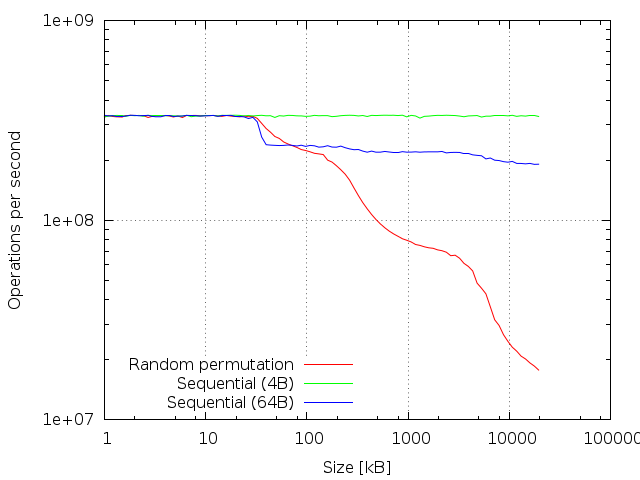
\includegraphics[scale=0.5]{results.png} 
% \end{center}
% \caption{Parallel Monte Carlo integration on Euler compute cluster.}
% \label{fig1}
% \end{figure}

\section{Question 2: Pararellelization}

Done as instructed and tested for correctness. Marginal improvement.\\

% \begin{figure}[H]
% \begin{tabular}{ccccc}
% \subfloat[Component 0]{\includegraphics[width = 1.1in]{lin_component_0.eps}} &
% \subfloat[Component 1]{\includegraphics[width = 1.1in]{lin_component_1.eps}} &
% \subfloat[Component 2]{\includegraphics[width = 1.1in]{lin_component_2.eps}} &
% \subfloat[Component 3]{\includegraphics[width = 1.1in]{lin_component_3.eps}} &
% \subfloat[Component 4]{\includegraphics[width = 1.1in]{lin_component_4.eps}} \\
% \subfloat[Component 5]{\includegraphics[width = 1.1in]{lin_component_5.eps}} &
% \subfloat[Component 6]{\includegraphics[width = 1.1in]{lin_component_6.eps}} &
% \subfloat[Component 7]{\includegraphics[width = 1.1in]{lin_component_7.eps}} &
% \subfloat[Component 8]{\includegraphics[width = 1.1in]{lin_component_8.eps}} &
% \subfloat[Component 9]{\includegraphics[width = 1.1in]{lin_component_9.eps}} 
% \end{tabular}
% \caption{10 Principal components of MNIST data set obtained from single linear hidden layer.}
% \label{fig:1}
% \end{figure}


\section{Question 3: Tweaking hyper-parameters}


I first of all changed the batch size from 512 to 128 and then went with the
following architecture:

\begin{itemize}
\item Conv2D layer: Filter size: $6 \times 6$, filter depth: $8$, strides: $2, 2$, output: $12\times12\times8$
\item LeakyReLU
\item Conv2D layer: Filter size: $5 \times 5$, filter depth: $16$, strides: $1, 1$, output: $8\times8\times16$
\item LeakyReLU
\item Conv2D layer: Filter size: $4 \times 4$, filter depth: $32$, strides: $1, 1$, output: $5\times5\times32$
\item LeakyReLU
\item Conv2D layer: Filter size: $3 \times 3$, filter depth: $64$, strides: $2, 2$, output: $2\times2\times64$
\item LeakyReLU
\item Conv2D layer: Filter size: $2 \times 2$, filter depth: $128$, strides: $1, 1$, output: $1\times1\times128$
\item LeakyReLU
\item Flatten to fully connected linear layer: Size: 128
\item LeakyReLU
\item Fully connected linear layer: Size: 10
\item SoftMax
\end{itemize}

Training over the same 50 epochs and overfitting a bit, a test set MSE of 0.053001
and a test set precision of 0.985377 were achieved with early stopping after 42 epochs.
This is quite a bit better than the untuned test results after 50 epochs (MSE:0.107567 precision:0.966900).

% \begin{figure}[H]
% \begin{tabular}{ccccc}
% \subfloat[Component 0]{\includegraphics[width = 1.1in]{component_0.eps}} &
% \subfloat[Component 1]{\includegraphics[width = 1.1in]{component_1.eps}} &
% \subfloat[Component 2]{\includegraphics[width = 1.1in]{component_2.eps}} &
% \subfloat[Component 3]{\includegraphics[width = 1.1in]{component_3.eps}} &
% \subfloat[Component 4]{\includegraphics[width = 1.1in]{component_4.eps}} \\
% \subfloat[Component 5]{\includegraphics[width = 1.1in]{component_5.eps}} &
% \subfloat[Component 6]{\includegraphics[width = 1.1in]{component_6.eps}} &
% \subfloat[Component 7]{\includegraphics[width = 1.1in]{component_7.eps}} &
% \subfloat[Component 8]{\includegraphics[width = 1.1in]{component_8.eps}} &
% \subfloat[Component 9]{\includegraphics[width = 1.1in]{component_9.eps}} i\\
% \subfloat[-Component 0]{\includegraphics[width = 1.1in]{component_10.eps}} &
% \subfloat[-Component 1]{\includegraphics[width = 1.1in]{component_11.eps}} &
% \subfloat[-Component 2]{\includegraphics[width = 1.1in]{component_12.eps}} &
% \subfloat[-Component 3]{\includegraphics[width = 1.1in]{component_13.eps}} &
% \subfloat[-Component 4]{\includegraphics[width = 1.1in]{component_14.eps}} \\
% \subfloat[-Component 5]{\includegraphics[width = 1.1in]{component_15.eps}} &
% \subfloat[-Component 6]{\includegraphics[width = 1.1in]{component_16.eps}} &
% \subfloat[-Component 7]{\includegraphics[width = 1.1in]{component_17.eps}} &
% \subfloat[-Component 8]{\includegraphics[width = 1.1in]{component_18.eps}} &
% \subfloat[-Component 9]{\includegraphics[width = 1.1in]{component_19.eps}} 
% \end{tabular}
% \caption{10 Principal components of MNIST data set obtained from three hidden layers with $\tanh$ activation function.}
% \label{fig:2}
% \end{figure}





\end{document}